\documentclass{article}
\usepackage{graphicx} % Required for inserting images
\usepackage[utf8]{inputenc}
\usepackage[russian]{babel}
\usepackage{enumitem}
\usepackage[T2A]{fontenc}
\usepackage{tocloft}
\usepackage{hyperref} 
\usepackage{tikz}
\usepackage{graphicx}

\renewcommand{\contentsname}{}

\title{Дизайн документ\\  «Escape the Matrix»}
\author{\\Куракина Юлия Вячеславовна}
\date{Ноябрь 2024}

\begin{document}

\maketitle

\tableofcontents 

\newpage
\section{Введение}

Данный документ описывает игру \textbf{«Escape the Matrix»}.\\ \\Содержание документа приведено на 1-2 страницах. \\Данный документ не является документом в форматах «EULA» или «Terms Of Use», он также не является коммерческой тайной. \\Документ написан на основании информации в общем доступе, полученной с веб-сервиса «GitHub»: \url{https://github.com/JuliaK434/Escape-the-Matrix} \\Документ менялся в период с ноября 2024 по апрель 2025 года.
\\Команда гейм-дизайнеров документа: Куракина Юлия Вячеславовна.\\Разработчики игры \textbf{«Escape the Matrix»}: Куракина Юлия Вячеславовна, Сергеев Максим Викторович, Дрямин Даниил Александрович. \\Сокращения и определения используются на основании документа \textbf{"Стандарт ГОСТ Р 53114-2008 «Защита информации. Обеспечение информационной безопасности в организации. Основные термины и определения»"}, других равносильных документов, также в документе могут использоваться общепринятые в обществе сокращения и определения. \\Дополнительных сведений для прочтения дизайн документа \textbf{не требуется}.

\newpage

\section{Концепция}

\paragraph{\textbf{Почему стоит обратить внимание на дизайн-документ:}}
Данный дизайн-документ является единственным в своём роде описанием игры «Escape the Matrix». Пользователь может ознакомиться с уникальностью данного проекта и протестировать продукт по вышеуказанной ссылке на «GitHub». Рекомендуется к прочтению тем, кто хочет ознакомиться с лором игры, её детальным функционалом и этапами разработки.
\paragraph{\textbf{Сюжет:}}
\textit{Главный герой игры — программист по имени Нуль, который неожиданно осознает, что живет внутри симуляции (Матрицы). Чтобы обрести свободу, ему нужно решить серию головоломок, каждая из которых приближает его к выходу из системы. По мере прохождения игрок узнает фрагменты истории персонажа и раскрывает тайны Матрицы.
}

\subsection{Введение}

\paragraph{\textbf{Суть игры:}}
"Escape the Matrix" — это головоломка с элементами квеста, где игрок должен анализировать окружение, находить скрытые подсказки и решать логические задачи, чтобы выбраться из виртуального мира. Игра сочетает атмосферу киберпанка с механиками, вдохновленными "Portal" и "Braid".

\subsection{Жанр и аудитория}
\begin{itemize}
\item 2D-головоломка, квест с элементами паззл-платформера.
\item Изометрическая игра – камера смотрит строго сверху, практически не меняя своего ракурса.
\end{itemize}

\subparagraph{Сеттинг:} Виртуальный мир, полный загадок.
\subparagraph{Целевая аудитория:} 16+ 
\begin{itemize}
\item Любящие интеллектуальные испытания.
\item Поклонники антиутопий, киберпанка и научной фантастики.
\item Те, кто ценит нарратив через геймплей, а не через длинные кат-сцены.
\end{itemize}
\subsection{Основные особенности игры}
USP – unique sellingpoints или ключевые особенности игры заключаются в ярком, неоновом, местами темном и фантастическим дизайне уровней. Простота и ясность "геймплея" добавляют особую атмосферу в прохождении, а нарастание сложности вызывает любопытство и интерес к финалу игры.
Также игра очень разнообразна на головоломки, что позволит любому игроку прокачать логику. 

\subparagraph{Обьём игры расчитан на 30 минут - 1 час}
\begin{enumerate}
    \item 
\end{enumerate}

\subsection{Описание игры}
Игрок перемещается по абстрактным локациям, напоминающим цифровые лабиринты, где стены, платформы и объекты подчиняются "правилам системы". Чтобы продвинуться, нужно:
\begin{enumerate}
\itemНаходить скрытые символы и коды.
\itemАктивировать переключатели в правильном порядке.
\itemИспользовать знания в написании кода.
\itemВзаимодействовать с ошибками в матрице (глитчи, аномалии).
\end{enumerate}
Финал игры — выход из симуляции, но открытый финал оставляет вопрос: реальность ли ждет героя снаружи?
\paragraph{Элементы управления:}
Движение вправо/влево: стрелки -> <- на клавиатуре, а также кнопками "A" и "D" соответственно.\\
Движение вверх/вниз: кнопками "W" и "S" соответственно.
  Прыжок: клавиша пробел.\\
    Пауза: клавиша esc.\\
      Главное меню: кнопки "«Значок Play»", "«Значок Настройки", "Значок Выход из игры".

\subparagraph{Задача игрока:} Дойти до конца, постепенно решая головоломки.

\subsection{Предпосылки создания}
Проект разрабатывается как демонстрация навыков геймдизайна и работы с движком Unity. Вдохновившись фильмом "Матрица", а так же такими играми как:  "Portal", "The Talos Principle", "Antichamber", нашей команде захотелось создать компактную, но насыщенную головоломку, где каждая механика работает на атмосферу и сюжет.

\subsection{Платформа}

\begin{center}
    \begin{tabular}{|p{4cm}|p{4cm}|p{6cm}|}
    \hline
      \textit{\textbf {Требования}}   & \textit{\textbf {Минимальные}}  & \textit{\textbf {Рекомендуемые}}  \\
      [0.5ex]
      \hline 
        \textit{\textbf {Операционная система}} & ОС Windows 7 (64-bit) & ОС Windows 11 (64-bit)\\
        \hline 
         \textit{\textbf {Процессор}} & Intel Core 2 Duo & Intel Core i3 или лучше\\
         \hline
         \textit{\textbf {ОЗУ}} & 2 ГБ & 4 ГБ\\
         \hline
         \textit{\textbf {Свободное место на HDD}} & 1 ГБ& 2 ГБ\\
         \hline
         \textit{\textbf {Видео карта}} & Встроенная видеокарта с поддержкой DirectX 9 & видеокарта с поддержкой DirectX 11 или выше\\
         \hline
         \textit{\textbf {Звуковая карта}} & Любая совместимая с Windiws & Любая совместимая с Windiws\\
         \hline
         \textit{\textbf {Управление}} & Клавиатура и мышь/трекпад & Клавиатура и мышь/трекпад\\ 
         \hline  
         \textit{\textbf {Unity}} & Версия Unity 6 (6000.0.23f1) &Версия Unity 6 (6000.0.23f1)\\ [1ex]
         \hline  
    \end{tabular}
\end{center}

\newpage
\section{Функциональная спецификация}

\subsection{Принципы игры}

\subsubsection{Суть игрового процесса}

\subsubsection{Ход игры и сюжет}

\subsection{Физическая модель}

\subsection{Персонаж игрока}
Нуль (Null) – минималистично и идеально для цифрового мира.

\subsection{Элементы игры}

\subsection{«Искусственный интеллект»}

\subsection{Интерфейс пользователя}

\subsubsection{Блок-схема}

\subsubsection{Функциональное описание и управление}

\subsubsection{Объекты интерфейса пользователя}

\subsection{Графика и видео}

\subsubsection{Общее описание}

\subsubsection{Двумерная графика и анимация}


\subsubsection{Анимационные вставки}

\subsection{Звуки и музыка}

\subsubsection{Общее описание}

\subsubsection{Звук и звуковые эффекты}

\subsubsection{Музыка}

\subsection{Описание уровней}
\begin{enumerate}[label=\arabic*., leftmargin=*]
    \item \textbf{1 уровень}\\
    \textbf{Начало}\\
    ГГ просыпается у себя в спальне и первым делом решает задачку, что ему одеть (Чтобы другие оценили и не засмеяли его - ГГ должен дать комментарии сам по поводу одежды).\\Смысл - человек находящийся в матрице боится быть самим собой, боится быть высмеянным или же не таким как все. Мини - игра для квеста: распределить одежду по цветам радуги.
\\ \textbf{Город}\\
ГГ в городе выполняет задания от его коллег. Находит ошибки в коде, считает матрицу, отгадывает что означает слово на русском языке из фрагмента фильмов на англ. (Матрица или бойцовский клуб)\\Смысл - развиваться всесторонне, люди в матрице считают, что они хороши лишь в одном. ГГ должен подметить что у него не всё хорошо с английским.
\item \textbf{2-3 уровень}\\
Повторяется принцип и локации 1-го уровня. С каждым уровнем сложность квестов повышается.
\item \textbf{4 уровень}\\
\\ \textbf{Хобби по Фэнтези}\\
 ГГ играет в фэнтэзи игру, где решает пойти не к финишу а в другую сторону, где встречает первого босса. Смысл этого хобби - раскрыть в монологах ГГ его качества: оптимизм и вера в невозможное. При этом диалоги в схватке с боссом должны быть похожи на реальную жизнь.
 \item \textbf{5 уровень}\\
 \\ \textbf{Осознание}\\
 ГГ просыпается на его гейм. месте, к нему подходит персонаж из фильма "Матрица" и рассказывает всю правду, Задаёт вопрос кто ты? Игроку даётся возможность походить по локациям игры, изучить её на ответ на вопрос. Правильный ответ: \textbf{Личность}
  \\ \textbf{Перезагрузка}\\
  Мир перезагружается (в виде двоичного кода) и ГГ попадает в киберпанк мир, где его тестируют на агента матрицы. Игрок выполняет квесты.
\item \textbf{6 уровень}\\
\\ \textbf{Тесты}\\
Игрок проходит тесты в локациях киберпанка. В финале агент рассказывает ему реальное положение вещей: из матрицы невозможно выбраться, и тебе лишь остаётся понять её устройство. Игрок сражается с финальным боссом. После этого он просыпается за своим гейм. местом.
\\ \textbf{Свободный мир}\\
ГГ открываются места прошлых локаций и открываются новые мини квесты (вне матрицы), где он понимает свои внутренние качества. ГГ остался жить свободно в матрице, так как понял кто он такой.Философский вопрос игроку: "Свободен ли ты?"
        \begin{itemize}
            \item Ответ "Да" - открывает выбор уровней
            \item Ответ "Нет" - статичный финальный экран
        \end{itemize}
\end{enumerate}

\subsubsection{Общее описание дизайна уровней}

\subsubsection{Диаграмма взаимного расположения уровней}
\begin{figure}[htbp]
\centering
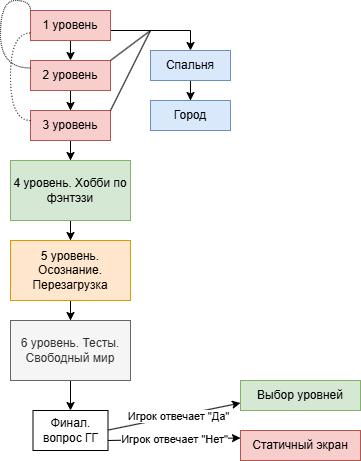
\includegraphics[width=0.8\textwidth]{Диаграмма взаимосвязей уровней} % Замените example-image на имя вашего файла
\caption{Диаграмма взаимного расположения уровней}
\label{fig:my_image}
\end{figure}

\subsubsection{График введения новых объектов}
\newpage

\section{Контакты}

\textbf{Куракина Юлия Вячеславовна} - Дизайн и программирование пользовательского интерфейса (UI/UX)(ivkurakina@edu.hse.ru)\\
\textbf{Сергеев Максим Викторович} - Реализация системы достижений и наград (mvsergeev@edu.hse.ru)\\
\textbf{Дрямин Даниил Александрович} - Тестирование и отладка.\\
\end{document}
